% Created by tikzDevice version 0.12.3.1 on 2021-11-19 21:15:37
% !TEX encoding = UTF-8 Unicode
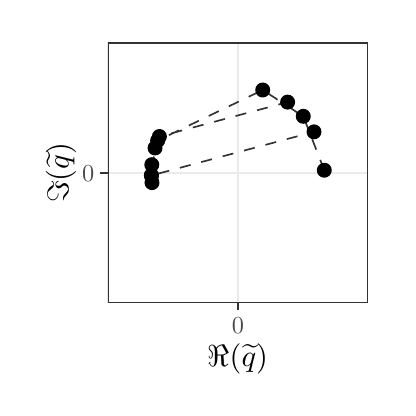
\begin{tikzpicture}[x=1pt,y=1pt]
\definecolor{fillColor}{RGB}{255,255,255}
\path[use as bounding box,fill=fillColor,fill opacity=0.00] (0,0) rectangle (130.09,130.09);
\begin{scope}
\path[clip] (  1.69,  0.00) rectangle (128.40,130.09);
\definecolor{drawColor}{RGB}{255,255,255}
\definecolor{fillColor}{RGB}{255,255,255}

\path[draw=drawColor,line width= 0.6pt,line join=round,line cap=round,fill=fillColor] (  1.69,  0.00) rectangle (128.40,130.09);
\end{scope}
\begin{scope}
\path[clip] ( 29.00, 30.69) rectangle (122.90,124.59);
\definecolor{fillColor}{RGB}{255,255,255}

\path[fill=fillColor] ( 29.00, 30.69) rectangle (122.90,124.59);
\definecolor{drawColor}{gray}{0.92}

\path[draw=drawColor,line width= 0.6pt,line join=round] ( 29.00, 77.64) --
	(122.90, 77.64);

\path[draw=drawColor,line width= 0.6pt,line join=round] ( 75.95, 30.69) --
	( 75.95,124.59);
\definecolor{drawColor}{RGB}{0,0,0}

\path[draw=drawColor,draw opacity=0.80,line width= 0.6pt,dash pattern=on 4pt off 4pt ,line join=round] (107.18, 78.58) --
	( 99.59, 98.06) --
	( 84.93,107.56) --
	( 46.96, 89.29) --
	( 46.03, 86.61) --
	( 44.72, 76.69) --
	(103.46, 92.45) --
	( 93.93,103.19) --
	( 47.60, 90.76) --
	( 44.85, 80.57) --
	( 44.91, 74.10) --
	( 44.72, 76.69);
\definecolor{drawColor}{RGB}{0,0,0}
\definecolor{fillColor}{RGB}{0,0,0}

\path[draw=drawColor,line width= 0.4pt,line join=round,line cap=round,fill=fillColor] (107.18, 78.58) circle (  2.50);

\path[draw=drawColor,line width= 0.4pt,line join=round,line cap=round,fill=fillColor] ( 99.59, 98.06) circle (  2.50);

\path[draw=drawColor,line width= 0.4pt,line join=round,line cap=round,fill=fillColor] ( 84.93,107.56) circle (  2.50);

\path[draw=drawColor,line width= 0.4pt,line join=round,line cap=round,fill=fillColor] ( 46.96, 89.29) circle (  2.50);

\path[draw=drawColor,line width= 0.4pt,line join=round,line cap=round,fill=fillColor] ( 46.03, 86.61) circle (  2.50);

\path[draw=drawColor,line width= 0.4pt,line join=round,line cap=round,fill=fillColor] ( 44.72, 76.69) circle (  2.50);

\path[draw=drawColor,line width= 0.4pt,line join=round,line cap=round,fill=fillColor] (103.46, 92.45) circle (  2.50);

\path[draw=drawColor,line width= 0.4pt,line join=round,line cap=round,fill=fillColor] ( 93.93,103.19) circle (  2.50);

\path[draw=drawColor,line width= 0.4pt,line join=round,line cap=round,fill=fillColor] ( 47.60, 90.76) circle (  2.50);

\path[draw=drawColor,line width= 0.4pt,line join=round,line cap=round,fill=fillColor] ( 44.85, 80.57) circle (  2.50);

\path[draw=drawColor,line width= 0.4pt,line join=round,line cap=round,fill=fillColor] ( 44.91, 74.10) circle (  2.50);

\path[draw=drawColor,line width= 0.4pt,line join=round,line cap=round,fill=fillColor] ( 44.72, 76.69) circle (  2.50);
\definecolor{drawColor}{gray}{0.20}

\path[draw=drawColor,line width= 0.6pt,line join=round,line cap=round] ( 29.00, 30.69) rectangle (122.90,124.59);
\end{scope}
\begin{scope}
\path[clip] (  0.00,  0.00) rectangle (130.09,130.09);
\definecolor{drawColor}{gray}{0.30}

\node[text=drawColor,anchor=base east,inner sep=0pt, outer sep=0pt, scale=  0.88] at ( 24.05, 74.61) {0};
\end{scope}
\begin{scope}
\path[clip] (  0.00,  0.00) rectangle (130.09,130.09);
\definecolor{drawColor}{gray}{0.20}

\path[draw=drawColor,line width= 0.6pt,line join=round] ( 26.25, 77.64) --
	( 29.00, 77.64);
\end{scope}
\begin{scope}
\path[clip] (  0.00,  0.00) rectangle (130.09,130.09);
\definecolor{drawColor}{gray}{0.20}

\path[draw=drawColor,line width= 0.6pt,line join=round] ( 75.95, 27.94) --
	( 75.95, 30.69);
\end{scope}
\begin{scope}
\path[clip] (  0.00,  0.00) rectangle (130.09,130.09);
\definecolor{drawColor}{gray}{0.30}

\node[text=drawColor,anchor=base,inner sep=0pt, outer sep=0pt, scale=  0.88] at ( 75.95, 19.68) {0};
\end{scope}
\begin{scope}
\path[clip] (  0.00,  0.00) rectangle (130.09,130.09);
\definecolor{drawColor}{RGB}{0,0,0}

\node[text=drawColor,anchor=base,inner sep=0pt, outer sep=0pt, scale=  1.10] at ( 75.95,  7.64) {$\Re(\widetilde q)$};
\end{scope}
\begin{scope}
\path[clip] (  0.00,  0.00) rectangle (130.09,130.09);
\definecolor{drawColor}{RGB}{0,0,0}

\node[text=drawColor,rotate= 90.00,anchor=base,inner sep=0pt, outer sep=0pt, scale=  1.10] at ( 14.76, 77.64) {$\Im(\widetilde q)$};
\end{scope}
\end{tikzpicture}
